\documentclass{beamer}
\usepackage[english]{babel}
\usepackage{color,hyperref}
\usepackage{amsmath}
\usepackage{amssymb}
\usepackage{amsfonts}
\usepackage{amsopn}
\usepackage{braket}
\usepackage{bbm}
\usepackage{dsfont}
\usepackage{kpfonts}
% \usepackage{mathabx}

\parindent=0cm


% Various new commands that ease typesetting math even further
% \newcommand{\assign}{\ensuremath{\coloneq}}
% \newcommand{\rassign}{\ensuremath{\eqcolon}}
\newcommand{\assign}{\ensuremath{:=}}
\newcommand{\rassign}{\ensuremath{=:}}

\newcommand{\of}[1]{\ensuremath{\left( #1 \right)}}
\newcommand{\ofs}[1]{\ensuremath{\left( #1 \right)}}

\newcommand{\norm}[1]{\ensuremath{\| #1 \|}}

\newcommand{\tmop}[1]{\ensuremath{\operatorname{#1}}}

\newcommand{\id}{\ensuremath{\mathds{1}}}
% \newcommand{\id}{\ensuremath{I}}


\newcommand{\conj}[1]{\ensuremath{\overline{#1}}}

\newcommand{\T}{\ensuremath{{}^{\textnormal{T}}}}
\newcommand{\herm}{\ensuremath{{}^{\textnormal{H}}}}

\newcommand{\ft}[1]{\ensuremath{\mathcal{F}\left(#1\right)}}
\newcommand{\ift}[1]{\ensuremath{\mathcal{F}^{-1}\left(#1\right)}}

\newcommand{\fft}[1]{\ensuremath{\mathtt{FFT}\left(#1\right)}}
\newcommand{\ifft}[1]{\ensuremath{\mathtt{IFFT}\left(#1\right)}}

\newcommand{\dotp}[2]{\ensuremath{\langle #1 , #2 \rangle}}

\newcommand{\bigO}[1]{\ensuremath{\mathcal{O}\left( #1 \right)}}

\newcommand{\mat}[1]{\ensuremath{\mathbf{#1}}}

% multi-indices
\newcommand{\mindex}[1]{\ensuremath{\underline{#1}}}

\newcommand{\laplace}{\ensuremath{\operatorname{\Delta}}}

% EOF

\usepackage{graphicx}
\usepackage{asymptote}
\usepackage[utf8x]{inputenc}

\mode<presentation>
{
  \usetheme{Montpellier}
  \setbeamercovered{transparent}
}

\title[Spawning in the non-adiabatic setting]{Spawning of wavepackets in 1D\\ non-adiabatic transitions}
\author[]{Raoul Bourquin\\~\\ Dr. Vasile Gr\u{a}dinaru\\ Prof. Dr. Ralf Hiptmair}

\date{Seminar for Applied Mathematics, ETH Zurich \\Spring semester 2011}

\newcommand{\burl}[1]{\footnotesize{\url{#1}}}

\beamertemplatenavigationsymbolsempty
%-----------------------------------------------------------------------------------------
\begin{document}

\begin{frame}
  \titlepage
\end{frame}


\begin{frame}{Outline}
  \tableofcontents
\end{frame}


\section{Introduction}
\subsection{Schrödinger equation, Potential and Initial Values}


\begin{frame}{Time-dependent Schrödinger equation}
  \begin{equation*} \label{eq:basics_tdse_semi}
    i \varepsilon^2 \frac{\partial}{\partial t} \Ket{\psi} = \underbrace{\left(T+V\right)}_{H} \Ket{\psi}
  \end{equation*}
  where
  \begin{equation*}
    T \assign - \frac{1}{2} \varepsilon^4 \frac{\partial^2}{\partial x^2} \qquad
    V \assign V\ofs{x}
  \end{equation*}
  \begin{itemize}
    \item Time evolution for a state $\Ket{\psi}$
    \item Kinetic operator $T$ and potential $V\left( x \right)$
    \item Semi-classical scaling $\varepsilon^2 \approx 10^{-2}, 10^{-3}, \ldots$
    \item Recover classical mechanics for $\varepsilon \rightarrow 0$
  \end{itemize}
\end{frame}


\begin{frame}{Wavefunction}{Representation of the wavefunction}
  \begin{itemize}
    \item Separation of variables
    \item Basis set expansion
    \begin{itemize}
      \item very successful idea $\rightarrow$ Roothaan equations in Hartree-Fock
    \end{itemize}
  \end{itemize}
  \begin{align*}
    \psi\ofs{x,t} & = \sum_k c_k\ofs{t} \phi_k\ofs{x} \\
                     & = \sum_k c_k\ofs{t} \phi_k\left[\Pi\ofs{t}\right]\ofs{x}
  \end{align*}
  Parameters:
  \begin{equation*}
    \Pi\ofs{t} \assign \{P\ofs{t}, Q\ofs{t}, p\ofs{t}, q\ofs{t}\}
  \end{equation*}
  Expansion coefficients:
  \begin{equation*}
    c\ofs{t} \assign \ofs{c_0\ofs{t}, \ldots, c_K\ofs{t}}
  \end{equation*}
\end{frame}


\begin{frame}{Semiclassical wavepackets}{Definition of the basis functions}
  \begin{itemize}
    \item Basis functions: product of a Gaussian times a polynomial
  \end{itemize}
  \begin{equation*} \label{eq:hagedorn_groundstate_1d}
  \phi_0 \ofs{x} \assign
  \left(\pi\varepsilon^2\right)^{-\frac{1}{4}} Q^{-\frac{1}{2}}
  \exp \left(
      \frac{i}{2\varepsilon^2} PQ^{-1}\left(x-q\right)^2
      + \frac{i}{\varepsilon^2} p\left(x-q\right)
  \right)
  \end{equation*}
  \begin{itemize}
    \item Parameters $P \in \mathbb{C}$, $Q \in \mathbb{C}$
    \item Position $q \in \mathbb{R}$ and momentum $p \in \mathbb{R}$
    \item Construct $\phi_k$ by applying the \emph{raising operator} $\mathcal{R}$
  \end{itemize}
  \begin{equation*}
    \phi_k \assign \frac{1}{\sqrt{k!}} \mathcal{R}^k \phi_0
  \end{equation*}
  \begin{itemize}
    \item $\{\phi_i\}_i$ complete basis of $L^2$ for fixed $P$, $Q$, $p$, $q$
  \end{itemize}
\end{frame}


\section{Semiclassical wavepackets}


\begin{frame}{Semiclassical wavepackets}{Definition of a wavepacket}
  \begin{itemize}
    \item General wavepacket as linear combination
  \end{itemize}
  \begin{equation*} \label{eq:hawp_def_single}
    \Phi\of{x} \assign e^{\frac{iS}{\varepsilon^2}} \sum_{k=0}^{K} c_k \phi_k \of{x}
  \end{equation*}
  \begin{itemize}
    \item In theory $K = \infty$, practically $K \leq 512$
    \item Time propagation of wavepackets:
    \begin{itemize}
      \item propagate parameters $P$, $Q$, $p$, $q$
      \item propagate coefficients $\{c_i\}_i$
    \end{itemize}
    \item \emph{Wavepackets stay in this mathematical form}
    \item Explicit algorithm $\rightarrow$ my Bachelor Thesis
  \end{itemize}
\end{frame}


\begin{frame}{Non-adiabatic potentials}
  \begin{itemize}
    \item Potential $V\ofs{x}$ with \emph{multiple} energy levels $\lambda_i\ofs{x}$
    \item Wavepackets can \emph{jump} to other levels
    \item and \emph{split up} over different levels
    \item Energy levels do never cross
  \end{itemize}
  Very simple example 
  \begin{columns}
    \begin{column}[T]{0.5\textwidth}
      \begin{equation*}
        V\ofs{x} = \left[\begin{smallmatrix}\frac{1}{2} \tanh{\left (x \right )} & \delta\\\delta & - \frac{1}{2} \tanh{\left (x \right )}\end{smallmatrix}\right]
      \end{equation*}
      \begin{itemize}
        \item $0 < \delta \in \mathbb{R}$
      \end{itemize}
    \end{column}
    \begin{column}[T]{0.5\textwidth}
        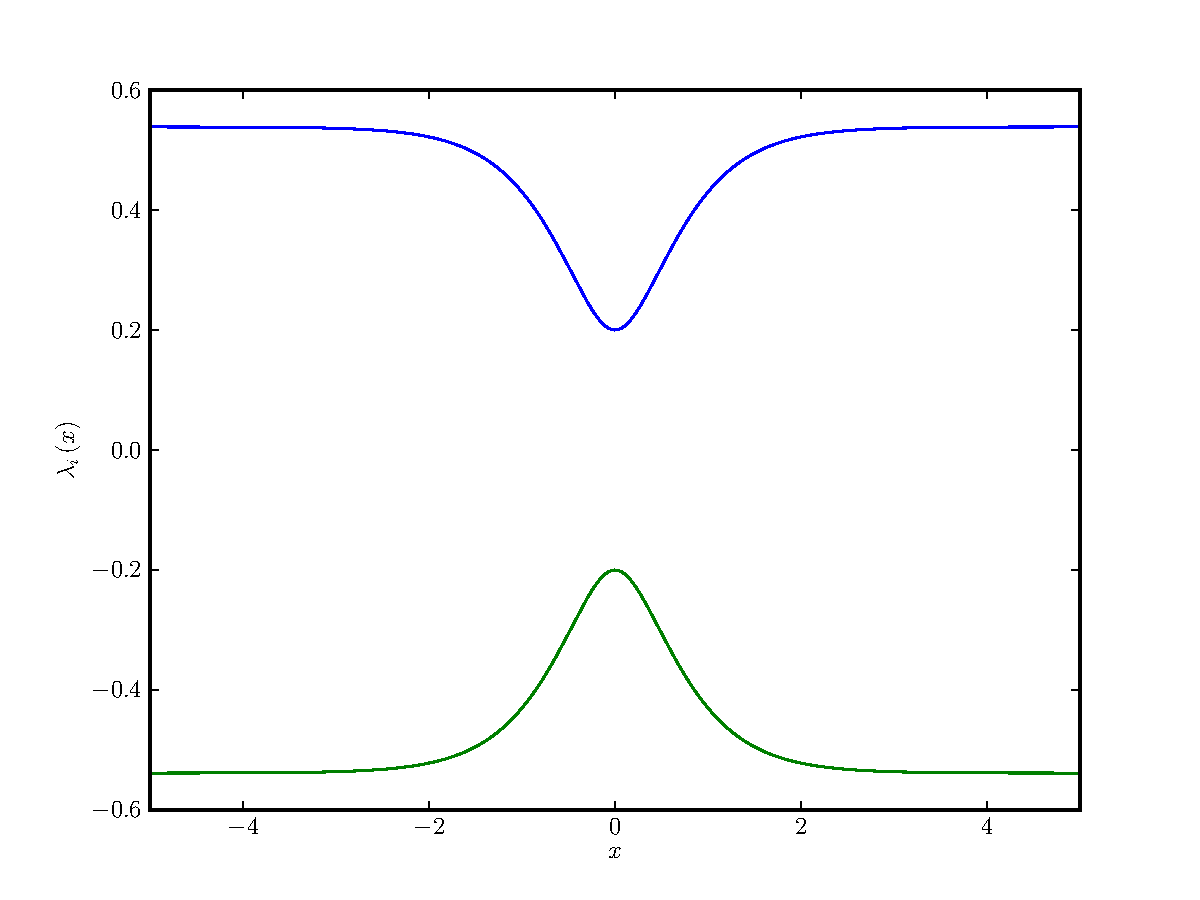
\includegraphics[scale=0.25]{./fig/delta_gap.pdf}
    \end{column}
  \end{columns}
\end{frame}


\begin{frame}{Non-adiabatic potentials}{Technical details}
  \begin{itemize}
    \item Potential $V\ofs{x}$ is a matrix
    \begin{itemize}
      \item Matrix valued TDSE
      \item Vector valued wavefunction
    \end{itemize}
    \item Wavepackets of the form:
    \begin{equation*}
      \Ket{\Psi} = \left(\begin{smallmatrix} \Phi_0 \\ \vdots \\ \Phi_{N-1} \end{smallmatrix} \right)
    \end{equation*}
    \item Usually homogeneous: same $\Pi$ for all $\Phi_i$
    \begin{itemize}
      \item \emph{really} a good idea?
      \item no, not always $\rightarrow$ \emph{spawning}
    \end{itemize}
  \end{itemize}
  \begin{center}
    Video of the time evolution without spawning
  \end{center}
\end{frame}


\section{Spawning}


\begin{frame}{Spawning}{Motivating example}
  \begin{figure}
    \centering
    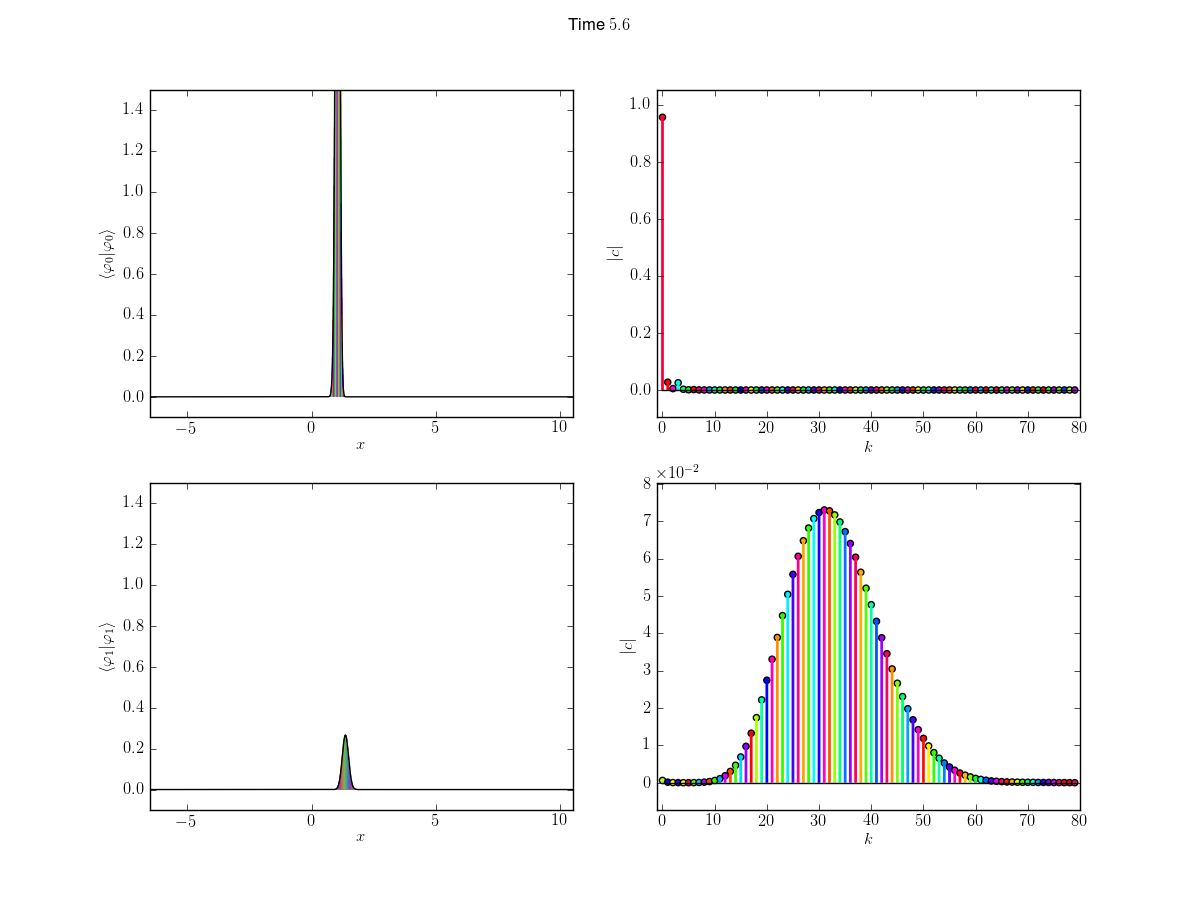
\includegraphics[width=0.8\linewidth]{./fig/spawn_motivation.png}
  \end{figure}
\end{frame}


\subsection{In the non-adiabatic setting}


\begin{frame}{Spawning}{In the non-adiabatic setting}
  \begin{itemize}
    \item Goal: reduce basis size $K$
    \begin{itemize}
      \item transformation to \emph{better} basis
    \end{itemize}
    \item Split up wavepackets: $\Ket{\Psi} = \Ket{\Psi_0} + \Ket{\Psi_1}$
    \item Each $\Ket{\Psi_i}$ has own set $\Pi_i$
    \begin{itemize}
      \item Important if $\Pi_0$ and $\Pi_1$ differ too much
      \item Allows smaller basis size for $\Psi_0$, $\Psi_1$
    \end{itemize}
    \item Important:
    \begin{itemize}
      \item Spawning may solve problems arising in \emph{long-time} simulations
      \item It does \emph{not} help with difficulties at the avoided crossing
    \end{itemize}
  \end{itemize}
\end{frame}


\begin{frame}{Spawning}{In the non-adiabatic setting}
  \begin{itemize}
    \item Split up wavepackets: $\Ket{\Psi} \approx \Ket{\Psi_0} + \Ket{\Psi_1} = \Ket{\Psi^\prime}$
    \item Reason: part $\Phi_1$ on lower level $\lambda_1$ travels faster
    \item Before split up by spawning:
    \begin{itemize}
      \item
      \begin{equation*}
        \Ket{\Psi} = \left(\begin{smallmatrix} \Phi_0 \\ \Phi_1 \end{smallmatrix} \right)
      \end{equation*}
      \item Single set $\Pi$ for both $\Phi_i$
      \item Probably big basis necessary: $K$ is large
    \end{itemize}
    \item After split up by spawning:
    \begin{itemize}
      \item
      \begin{equation*}
        \Ket{\Psi^\prime} = \left(\begin{smallmatrix} \Phi_0^\prime \\ 0 \end{smallmatrix} \right)
                          + \left(\begin{smallmatrix} 0 \\ \Phi_1^\prime \end{smallmatrix} \right)
      \end{equation*}
      \item Each $\Phi_i^\prime$ has own parameter set $\Pi_i$
      \item Hopefully each $\Psi_i^\prime$ needs only much smaller basis
    \end{itemize}
  \end{itemize}
\end{frame}


\subsection{Mathematical problem description and details}


\begin{frame}{Spawning}{Mathematical problem description}
  \emph{Given a linear combination} $\sum_{k=\alpha}^\beta c_k \phi_k\left[\Pi\right]\ofs{x}$
  \emph{with} $\alpha \geq 0$ \emph{and} $\beta \leq K$ \emph{find
  a new, optimal basis of} $L^2$. \emph{More precisely, find a new set}
  $\tilde{\Pi}$ \emph{of parameters.} \emph{Then do a basis expansion
  in the new basis} $\sum_{k=\alpha}^\beta \tilde{c}_k \phi_k [\tilde{\Pi}]$
  \emph{resulting in new coefficients} $\tilde{c}$.
\end{frame}


\begin{frame}{Spawning}{Parameter estimation in detail}
  \begin{itemize}
    \item A fragment: $w \assign \sum_{k=\alpha}^\beta c_k \phi_k$
    \item Estimate optimal $\tilde{\Pi}$ for $w$ via expectation values
  \end{itemize}
  \begin{align*}
    \tilde{q} & \assign \frac{\Braket{w | x | w}}{\Braket{w|w}}
              = \frac{\sqrt{2 \varepsilon^2}}{\sum_{k=\alpha}^\beta \conj{c_k} c_k} \Re \left(Q \sum_{k=\alpha+1}^\beta \conj{c_k} c_{k-1} \sqrt{k} \right) + q \\
    \tilde{p} & \assign \frac{\Braket{w | -i \varepsilon^2 \frac{\partial}{\partial x} | w}}{\Braket{w|w}}
              = \frac{\sqrt{2 \varepsilon^2}}{\sum_{k=\alpha}^\beta \conj{c_k} c_k} \Re \left(P \sum_{k=\alpha+1}^\beta \conj{c_k} c_{k-1} \sqrt{k} \right) + p
  \end{align*}
  \begin{itemize}
    \item Similar procedure for $\tilde{Q}$ and $\tilde{P}$
    \item Non-adiabatic setting: $\Phi_1 \equiv w$ and $\alpha=0$, $\beta=K$
  \end{itemize}
\end{frame}


\begin{frame}{Spawning}{Change of basis}
  \begin{itemize}
    \item Find the expansion coefficients $\tilde{c}_k$
    \item Different strategies possible
    \begin{itemize}
      \item \emph{Lumping}
      \item \emph{Basis projection}
      \item \ldots
    \end{itemize}
    \item Both have advantages and drawbacks
    \begin{itemize}
      \item \emph{Basis projection} is the cleaner solution
    \end{itemize}
  \end{itemize}
\end{frame}


\begin{frame}{Spawning}{Basis projection}
  \begin{itemize}
    \item Project $w$ to first $\mu$ new basis functions $\tilde{\phi}_k \assign \phi_k[\tilde{\Pi}]$
    \begin{equation*}
      \tilde{c}_i \assign \frac{\Braket{w|\tilde{\phi}_i}}{\Braket{w|w}}
    \end{equation*}
    \item Do these integrals with highly accurate quadrature
    \begin{equation*}
      \tilde{c}_i = \varepsilon \cdot Q_0 \sum_{r=0}^{R-1} \conj{\sum_{k=\alpha}^\beta c_k \phi_k\ofs{\gamma_r}} \cdot \tilde{\phi}_i \ofs{\gamma_r} \cdot \omega_r \,.
    \end{equation*}
    \item Finally assign the coefficients
    \begin{equation*}
    \begin{split}
      \tilde{c} & \assign
      \begin{pmatrix}
        \tilde{c}_0 & \cdots & \tilde{c}_{\mu} & \tilde{c}_{\mu+1} = 0 & \cdots & \tilde{c}_{\eta-1} = 0
      \end{pmatrix} \\
      \begin{pmatrix}
        c_\alpha & \cdots & c_\beta
      \end{pmatrix} & \assign 0 \,.
    \end{split}
    \end{equation*}
  \end{itemize}
\end{frame}


\begin{frame}{Spawning}{Spawning criteria}
  \begin{itemize}
    \item An oracle telling us if and when to spawn
    \begin{itemize}
      \item Spawn to early is \emph{very bad}
      \item Spawn to late is of little risk
    \end{itemize}
  \end{itemize}
  \begin{columns}
    \begin{column}[T]{0.4\textwidth}
      \begin{center}
        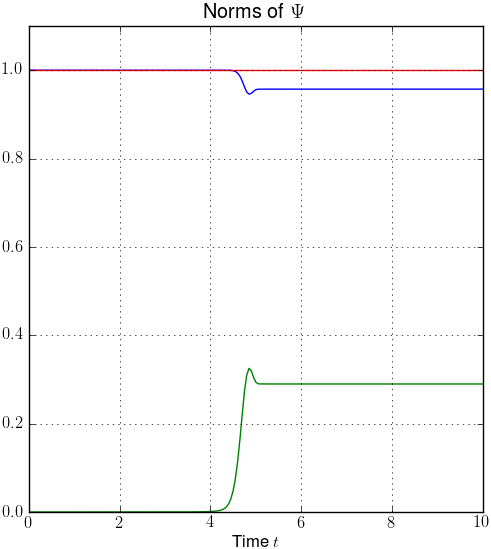
\includegraphics[scale=0.3]{./fig/norms_block0.png}
      \end{center}
    \end{column}
    \begin{column}[T]{0.6\textwidth}
      \begin{itemize}
        \item Simple threshold based criterion
        \begin{itemize}
          \item $\Braket{w,w} \geq \tau$
          \item asymptotic value $\approx \tau$
          \item but a priori unknown!
        \end{itemize}
        \item More advanced criteria possible
      \end{itemize}      
    \end{column}
  \end{columns}
\end{frame}


\section{Implementation}


\begin{frame}{Implementation}
  \begin{itemize}
    \item Implementation on top of \texttt{WaveBlocks}
    \begin{itemize}
      \item My code framework from the Bachelor Thesis
      \item Currently about 8k lines of python code (core only)
      \item Highly modular and easily extendable
      \item Object oriented python code using \texttt{numpy} for numerics
    \end{itemize}
    \item Adding spawning algorithms was really easy
    \begin{itemize}
      \item Only 4 new classes
      \begin{itemize}
        \item Parameter estimation routines
        \item Change of basis routines
        \item Code that checks for spawning during time propagation
      \end{itemize}
      \item About 500 lines of new code (w/o data analysis and plotting)
    \end{itemize}
  \end{itemize}
  \begin{center}
    
\includegraphics[scale=1.0]{./fig/python-powered-w.pdf}
  \end{center}
\end{frame}


\section{An Example}


\begin{frame}{An example}{Estimated parameters}
  \begin{center}
    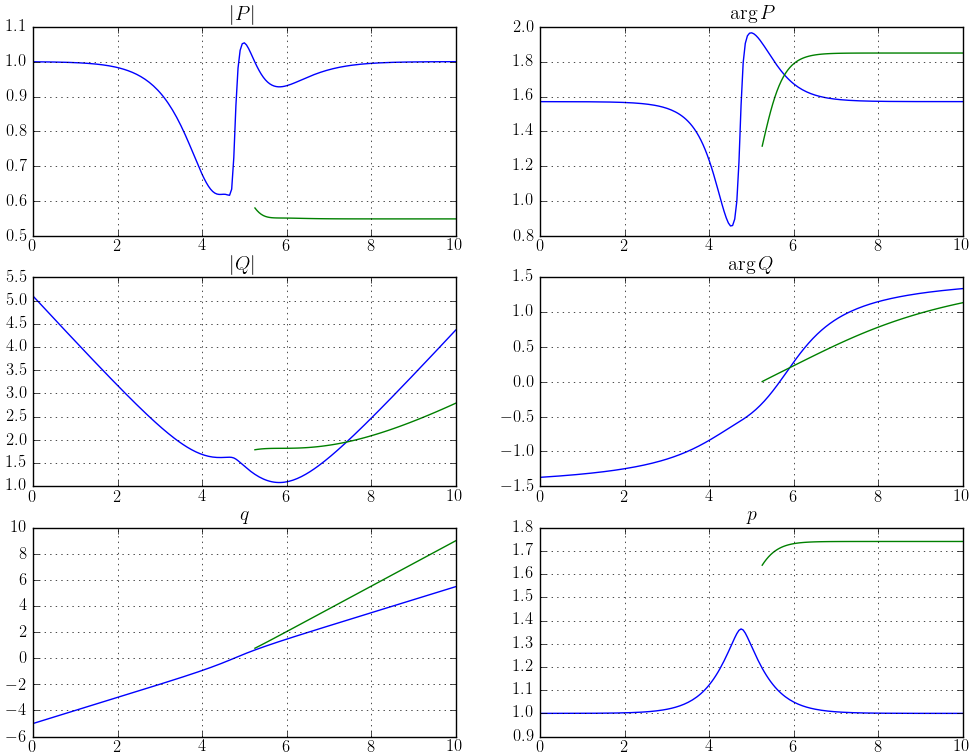
\includegraphics[scale=0.35]{./fig/wavepacket_parameters_estimation.png}
  \end{center}
\end{frame}


\begin{frame}{An example}{Norms}
  \begin{center}
    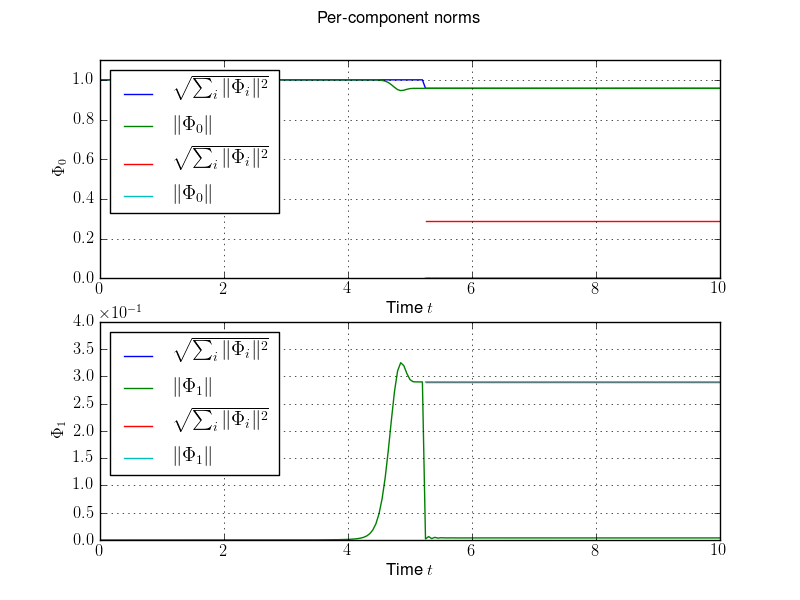
\includegraphics[scale=0.4]{./fig/norms_components_spawned.png}
  \end{center}
\end{frame}


\begin{frame}{An example}{Video}
  \begin{center}
    Video of the time evolution with spawning
  \end{center}
\end{frame}


\begin{frame}{An example}{Spawning error}
  \begin{center}
    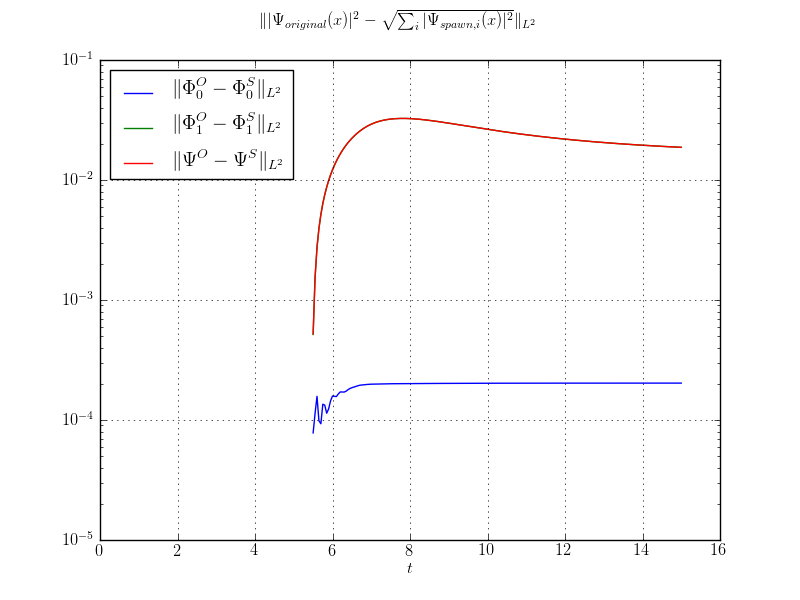
\includegraphics[scale=0.35]{./fig/spawn_error_sum_L2norm0.png}
  \end{center}
  \begin{itemize}
    \item \emph{Systematic} ways to reduce the spawning error
  \end{itemize}
\end{frame}


\section{Future work}


\begin{frame}{Current research}
  Refine spawning in the \emph{non-adiabatic} case
  \begin{itemize}
    \item Open issues with parameter estimation
    \item Can we improve the change of basis?
    \item Compare spawn criteria and find best one
    \item Propagation algorithm in case the interaction of\\
    the spawned packets can not be neglected (hard!)
    \item Adaptive basis size (almost done)
  \end{itemize}
\end{frame}


\section{End}


\begin{frame}{Thanks for your attention}
  \begin{center}
    Questions?    
  \end{center}
  \vspace{15pt}
  More information on the topic
  \begin{itemize}
    \item The full thesis:\\
    {\burl{http://n.ethz.ch/~raoulb/research/term_thesis/main.pdf}}
    \item The \texttt{WaveBlocks} source code:\\
    {\burl{http://waveblocks.origo.ethz.ch/}} \\
    {svn \burl{http://svn.origo.ethz.ch/waveblocks/}}
  \end{itemize}
\end{frame}

\end{document}
